% ****** Start of file apssamp.tex ******
%
%   This file is part of the APS files in the REVTeX 4.1 distribution.
%   Version 4.1r of REVTeX, August 2010
%
%   Copyright (c) 2009, 2010 The American Physical Society.
%
%   See the REVTeX 4 README file for restrictions and more information.
%
% TeX'ing this file requires that you have AMS-LaTeX 2.0 installed
% as well as the rest of the prerequisites for REVTeX 4.1
%
% See the REVTeX 4 README file
% It also requires running BibTeX. The commands are as follows:
%
%  1)  latex apssamp.tex
%  2)  bibtex apssamp
%  3)  latex apssamp.tex
%  4)  latex apssamp.tex
%
\documentclass[%
 preprint,
%superscriptaddress,
%groupedaddress,
%unsortedaddress,
%runinaddress,
%frontmatterverbose, 
%preprint,
%showpacs,preprintnumbers,
%nofootinbib,
%nobibnotes,
%bibnotes,
 amsmath,amssymb,
 aps,
%pra,
%prb,
%rmp,
%prstab,
%prstper,
%floatfix,
]{revtex4-1}

\usepackage{graphicx}% Include figure files
\usepackage{dcolumn}% Align table columns on decimal point
\usepackage{bm}% bold math
\usepackage{hyperref}% add hypertext capabilities
\usepackage[mathlines]{lineno}% Enable numbering of text and display math
\linenumbers\relax % Commence numbering lines
\usepackage{xcolor}

%\usepackage[showframe,%Uncomment any one of the following lines to test 
%%scale=0.7, marginratio={1:1, 2:3}, ignoreall,% default settings
%%text={7in,10in},centering,
%%margin=1.5in,
%%total={6.5in,8.75in}, top=1.2in, left=0.9in, includefoot,
%%height=10in,a5paper,hmargin={3cm,0.8in},
%]{geometry}

\begin{document}

%\preprint{APS/123-QED}

\title{Self consistency calculation for Pseudo Bogoliubov Landau levels}% Force line breaks with \\
\thanks{A footnote to the article title}%

\author{O\u{g}uz T\"{u}rker}
 \altaffiliation[Also at ]{Physics Department, Technical university of Dresden}%Lines break automatically or can be forced with \\
%%\author{Second Author}%
%% \email{Second.Author@institution.edu}
%%\affiliation{%
%% Authors' institution and/or address\\
%% This line break forced with \textbackslash\textbackslash
%%}%

%\collaboration{MUSO Collaboration}%\noaffiliation

%\author{Charlie Author}
% \homepage{http://www.Second.institution.edu/~Charlie.Author}
%\affiliation{
% Second institution and/or address\\
% This line break forced% with \\
%}%
%\affiliation{
% Third institution, the second for Charlie Author
%}%
%\author{Delta Author}
%\affiliation{%
% Authors' institution and/or address\\
% This line break forced with \textbackslash\textbackslash
%}%
%
%\collaboration{CLEO Collaboration}%\noaffiliation

\date{\today}% It is always \today, today,
             %  but any date may be explicitly specified

\begin{abstract}
%In recent works it is shown that in time reversal breaking weyl semi metals modulating the node separation length by applying strain produces pseudo magnetic field and gives rise to landau levels. Also it is shown that the same effect can be achieved by applying superconductivity with spatially modulating order parameter, since the magnitude of the separation  bla bla bla.
\begin{description}
\item[Usage]
Secondary publications and information retrieval purposes.
\item[PACS numbers]
May be entered using the \verb+\pacs{#1}+ command.
\item[Structure]
You may use the \texttt{description} environment to structure your abstract;
use the optional argument of the \verb+\item+ command to give the category of each item. 
\end{description}
\end{abstract}

\pacs{Valid PACS appear here}% PACS, the Physics and Astronomy
                             % Classification Scheme.
%\keywords{Suggested keywords}%Use showkeys class option if keyword
                              %display desired
\maketitle

%\tableofcontents

\section{\label{sec:level1}Introduction}


\section{\label{sec:2}Pseudo-Landau levels  }
It is shown that  if a Weyl semi-metal becomes superconducting, the magnitude of the superconducting order parameter controls the separation of the Weyl nodes. Thus if our system have a superconductivity with spatially modulating order parameter, we expect to have spatially modulating separation length of the Weyl nodes.
In this section we quantitatively show our arguments, and in the following section we will calculate the superconducting order parameter self-consistently. We start adding s-wave superconductivity to a Weyl semi-metal. 
\begin{equation}
H=\sum_{\boldmath{k}}c^{\dagger}_{\mathbf{k}}[\mathbf{d(\mathbf{k})}\cdot\mathbf{\sigma}]c_{\mathbf{k}}+(\Delta_0c^{\dagger}_{\uparrow k}c^{\dagger}_{\downarrow -k}+h.c.) \label{eq:ham},
\end{equation}
where $c_k=(c_{\uparrow k},c_{\downarrow k})^{\text{T}}$, $\mathbf{d(\mathbf{k})}=-(\sum_{i}\cos(k_i)-\cos(k_0)-m_g,\sin(k_2),\sin(k_3))$, $m_g$ controls the size of the gap and we take it always positive $k_0$ controls the position of the Weyl nodes. We will denote the first term in eq(\ref{eq:ham}) as $H_0$. $H_0$ hosts Weyl nodes at $k=(\pm k_0,0,0)$ for $m_g=0$. If we let $m_g$, $k_0$ and $\Delta_0$ to be zero we would get a quadratic band touching at $\mathbf{k}=0$ and then if we let $\Delta_0>0$ this Dirac node  would be separated into two Weyl nodes. It is known that the Dirac node  can be transformed into a Weyl nodes either by breaking time reversal symmetry or inversion symmetry.  Time reversal symmetry can be broken by applying external magnetic field to the system with Dirac node. In our system we break time reversal symmetry by adding superconductivity thus, superconducting order parameter behaves like a pseudo-electromagnetic potential.[\textcolor{red}{Check this!}] If the superconducting order parameter spatially inhomogeneous then we would observe finite pseudo magnetic field. 

First we write \ref{eq:ham} as a Bogoliubov Hamiltonian such that
\begin{equation}
H_\textbf{bog}=\frac{1}{2}\sum_{k}\gamma^{\dagger}_{k}[\tau_3\otimes d({k_\parallel})\cdot\sigma_{\parallel}+\tau_0\otimes\sigma_3 d_3(k_3)+[\tau^{+}\Delta_0-\tau^{-}\Delta_0^*]\otimes \textbf{i}\sigma_2]\gamma_{k}+\text{const.}, \label{eq: boghaminkspac}
\end{equation}
where $\sigma_i$ are spin degree of freedom, $\tau_i$ are particle-hole degree of freedom, $\gamma_{k}=(c_{k\uparrow},c_{k\downarrow},c^{\dagger}_{-k\uparrow},c^{\dagger}_{-k\downarrow})^{\text{T}}$, $k_{\parallel}=(k_1,k_2)$ and $\sigma_{\parallel}=(\sigma_1,\sigma_2)$. In order to diagonalize eq.(\ref{eq: boghaminkspac}) in particle hole space we first make a canonical transformation in order to decouple $\sigma$ and $\tau $ degree of freedom , 
\begin{equation}
(c_{k\uparrow},c_{k\downarrow},c^{\dagger}_{-k\uparrow},c^{\dagger}_{-k\downarrow})^{\text{T}}\rightarrow (c_{k\uparrow},c_{k\downarrow},c^{\dagger}_{-k\uparrow},-c^{\dagger}_{-k\downarrow})^{\text{T}}
\end{equation}
then after diagonalizing in $\tau$ degree of freedom we get 
\begin{equation}
H_{\textbf{bog}}=\frac{1}{2}\sum_{k}\phi^{\dagger}_{k}\begin{bmatrix}
    d(k)\cdot \sigma+|\Delta_0|\sigma_1 & \mathbf{0} \\
    \mathbf{0} & d(k)\cdot \sigma-|\Delta_0|\sigma_1 
\end{bmatrix} \phi_{k} +\text{const.}\label{eq:bogks}
\end{equation}
We denote the upper(lower) block of eq(\ref{eq:bogks}) as $H_{+(-)}$. $H_{\pm}$ hosts two Weyl points  if $1<(2+\cos(k_0)+m_g\pm\Delta_0)<3$ and it is an insulator for $(2+\cos(k_0)+m_g\pm\Delta_0)>3$. We will let $k_0=0$ so only $H_{-}$ will host Weyl points and $H_{+}$ will be an insulator, and our system in total will host only two Weyl nodes. We add mass term to make on of the block Hamiltonian always an insulator, and in order to have a smooth transition from insulating phase to Weyl phase in the boundary of the finite slab.  The separation between two Weyl nodes is
\begin{equation}
b=2\cos^{-1}(\cos(k_0)-|\Delta_0|)
\end{equation}


For the next step we will write the Bogoliubov Hamiltonian with spatially inhomogeneous order parameter. We will assume that we have a slab in  direction $\hat{x}_2$ with $N$ sites and order parameter will be spatially inhomogeneous in in  direction $\hat{x}_2$ . Thus the separation of Weyl nodes becomes $b(x_2)=2\cos^{-1}(\cos(k_0)-|\Delta_0(x_2)|$, thus we have a pseudo magnetic field in $\hat{x}_3$ direction. In order to do so we first start with an Hamiltonian with quadratic interaction and then we will apply mean field theory. The Hamiltonian is given as,
\begin{equation}
H=H_0+\sum_{k_\perp ij}\frac{g_{ij}}{V}c^{\dagger}_{k_\perp i\uparrow}c^{\dagger}_{-k_\perp i\downarrow}c_{-k_\perp j\downarrow}c_{k_\perp j\uparrow}\label{eq:hint}
\end{equation}
where $k_{\perp}=(k_1,k_3)$ and $V$ is the volume of the system.
We can assume contact interaction by letting  $g_{ij}=-g_0\delta_{ij}$. We can apply a mean-field theory by defining 
\begin{equation}
\Delta_j=-\frac{g_0}{V}\sum_{k_\perp}\langle c_{-k_\perp j\downarrow}c_{k_\perp j\uparrow}\rangle_\textbf{th},\label{eq:scd}
\end{equation}
then we get, 
\begin{equation}
H=H_0+\sum_{k_\perp i}[\Delta_ic^{\dagger}_{k_\perp i\uparrow}c^{\dagger}_{-k_\perp i\downarrow}+\text{h.c.}] +\text{const.}\label{eq: scham}.
\end{equation}
We can write eq.(\ref{eq: scham}) in Bogoliubov Hamiltonian form,
\begin{equation}
H_{\textbf{bog}}=\frac{1}{2}\sum_{k_{\perp}}\psi^{\dagger}_{k_{\perp}}\begin{bmatrix}
    H(k_{\perp}) & \Delta \\
    \Delta^{\dagger} & -H(-k_{\perp})^{\text{T}} 
\end{bmatrix} \psi_{k_{\perp}}+\text{const.} \label{eq:hobog}
\end{equation}
where $\Delta$ is $2N\times2N$ block-diagonal matrix with blocks of $\textbf{i}\sigma_2 \Delta_i$, $H(k_{\perp})$ is position space representation of $H_0$,  $\psi_{i\sigma k_{\perp}}=c_{i\sigma k_{\perp}}$ and $\psi_{i+2N\sigma k_{\perp}}=c^{\dagger}_{i\sigma -k_{\perp}}.$ If we solve eq(\ref{eq:hobog}) with appropriate $\Delta_i$ we observe Landau levels. 

\begin{figure*}[h!]
\begin{center}
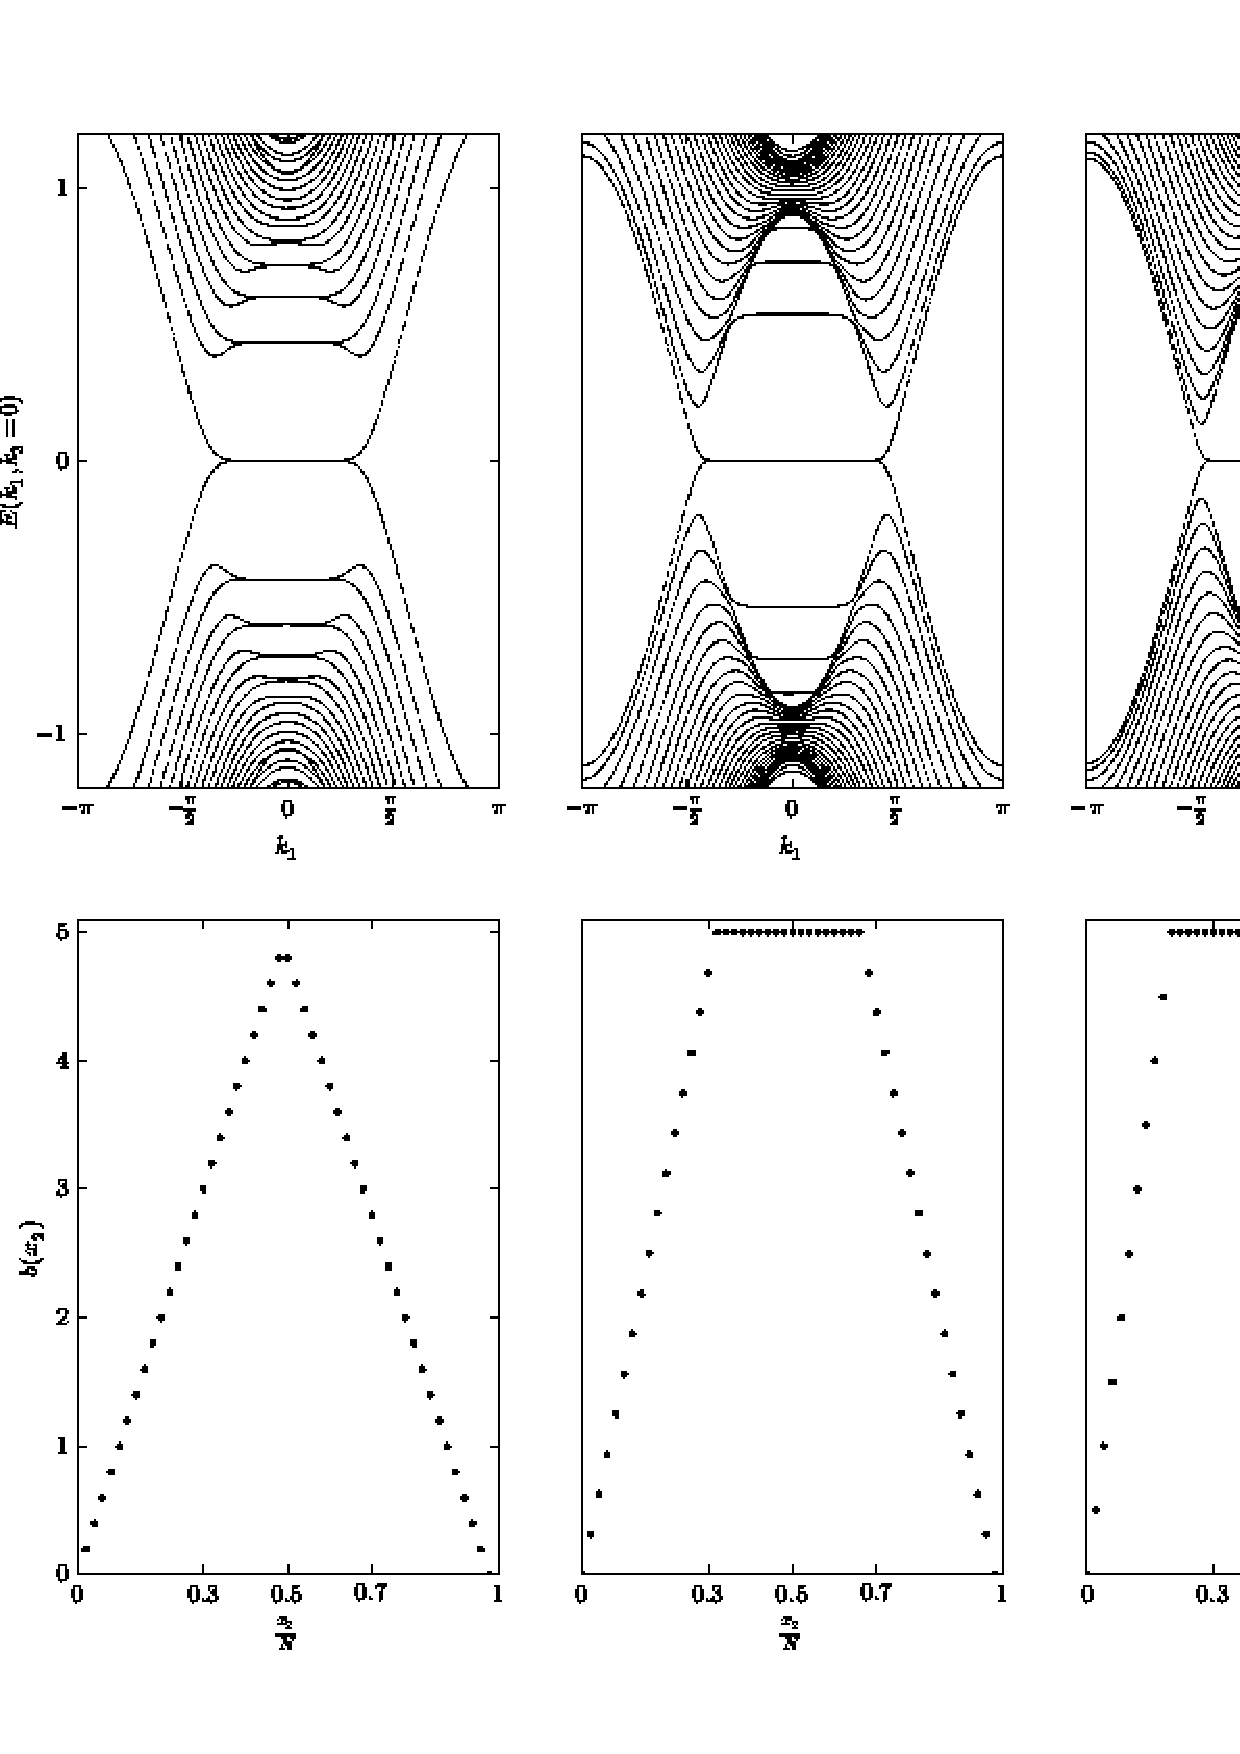
\includegraphics[width=1\textwidth]{lll.pdf}
\caption{I will  add comment}
\end{center}
\end{figure*}
\section{Self consistency equation}
The spatial inhomogeneity of the superconducting order parameter can be achieved may spatially modulating strain, temperature or chemical potential.  We will consider the latter case. We assume periodic boundary conditions, i.e. $\mu(i+n)=\mu(i)$ where $n$ is the number of sites in super-cell. The superconducting order parameter id
\begin{equation}
\Delta_{\alpha_i}=\frac{1}{V}\sum_{k}g(k)\langle c_{-k \alpha_i\downarrow}c_{k \alpha_i\uparrow}\rangle_\text{th},\label{eq:scdmu}
\end{equation}
where $\alpha_i$ is the index of the lattice site in the super-cell and runs from $0$ to $n$. The particle and hole eigenstates states of the Bogoliubov Hamiltonian are
\begin{equation}
\begin{bmatrix}
    H(k) & \Delta \\
    \Delta^{\dagger} & -H(-k)^{\text{T}} 
\end{bmatrix}
\begin{bmatrix}
    u_{m}(k)  \\
    v_{m}(k) 
\end{bmatrix}
=E_{m}(k) \begin{bmatrix}
    u_{m}(k)  \\
    v_{m}(k) 
\end{bmatrix}
\label{eq:particle}
\end{equation}
\begin{equation}
\begin{bmatrix}
    H(k) & \Delta \\
    \Delta^{\dagger} & -H(-k)^{\text{T}} 
\end{bmatrix}
\begin{bmatrix}
    v^{*}_{m}(-k)  \\
    u^{*}_{m}(-k) 
\end{bmatrix}
=-E_{m}(-k) \begin{bmatrix}
    v^{*}_{m}(-k)  \\
    u^{*}_{m}(-k) 
\end{bmatrix}
\label{eq:hole}
\end{equation}
where $m$ is the superconducting band index, $u$ and $v$ are $2n\times1$ sized column vectors.
If we diagonalize the Bogoliubov Hamiltonian by using eq(\ref{eq:particle}) and eq(\ref{eq:hole}), we have
\begin{align}
c_{ k \alpha_i\uparrow}=\sum_{m}u_{m\uparrow\alpha_i}(k)\gamma_{km}+v^{*}_{\alpha_i m\uparrow }(-k)\gamma^{\dagger}_{-km}\\c_{ -k \alpha_i\downarrow}=\sum_{m}u_{m\downarrow\alpha_i}(-k)\gamma_{-km}+v^{*}_{\alpha_i m\downarrow}(k)\gamma^{\dagger}_{km}
\end{align}
Thus the self consistency condition  at absolute zero is
\begin{equation}
\Delta_{\alpha_i}=\frac{1}{V}\sum_{k m}g(k)u_{m\downarrow\alpha_i}(k)v^{*}_{\alpha_i m\uparrow}(k)\label{eq:sceq}
\end{equation}
with
\begin{equation}
g(k)=\left\{
\begin{aligned}
&-g_0,&& \text{for }|\xi_k|\leq\omega_d \\
& 0, && \text{otherwise} 
\end{aligned} \right.
\end{equation}
where $\xi_k$ [\textcolor{red}{there are 2n $\xi_k$  for which one we should check this condition! }]are eigenvalues of $H(k)$ and $\omega_d$ is the Deby frequency. The self consistency equation can be solved analytically for small $n$ and numerically for large $n$. If solve for constant $\mu$ eq(\ref{eq:sceq}) numerically we get exponential dependency of $\Delta$ to $\mu$.
\begin{figure}[h!]
\begin{center}
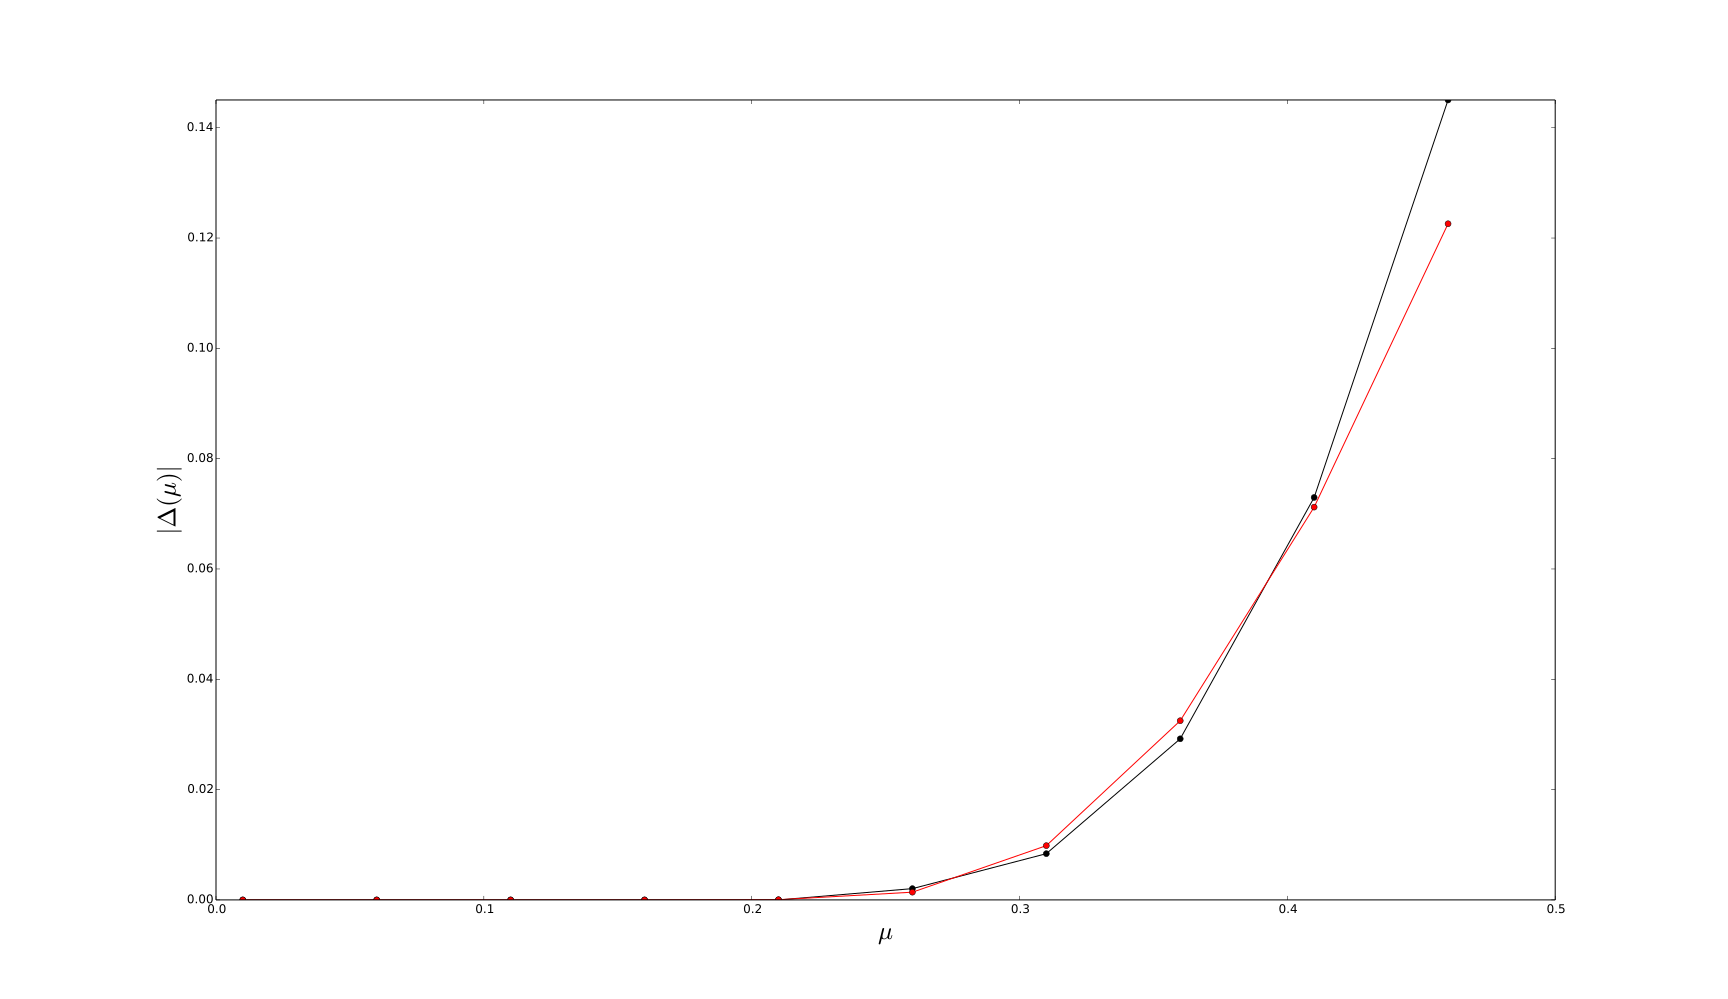
\includegraphics[width=1\textwidth]{delta_vs_mu_prop.pdf}
\caption{This is calculated with $n=2$, $\omega_d=0.2$, $g_0=100$, $k_0=\frac{{\pi}}{3}$, $\delta\mu=0.05$ and $\delta k=0.2$. Red is analytic and black is numeric. The $g_0$ is unphysically high because otherwise both of them(numeric and analytic solution) would be zero in the regime of the  approximation of  the analytic calculation  holds.}
\end{center}
\end{figure}
\begin{figure}[h!]
\begin{center}
\includegraphics[width=1\textwidth]{dos_anl_vs_num.pdf}
\caption{Density of states}
\end{center}
\end{figure}
\textcolor{red}{We can add an analytic calculation of dos and $\Delta$ for $n=2$ here.}

For the next step we will solve the self consistency equation for spatially inhomogeneous $\mu$.
\begin{figure}[h!]
\begin{center}
\includegraphics[width=1\textwidth]{debye_vs_delta.pdf}
\caption{I think this  occurs because of the finite size of $k$ here $\mu=0.4$}
\end{center}
\end{figure}


\end{document}

%
% ****** End of file apssamp.tex ******
